\section{Servidor Frontend - Ember.JS}

O servidor \textit{frontend} do subsistema, responsável pela visualização dos
dados, tinha como resultados esperados uma aplicação que pudesse prover a
visualização dos sinais referentes a um determinado paciente, baseado nas
informações recebidas do servidor de \textit{backend}. Devido à necessidade de
uma certa dinamicidade na apresentação desses dados, foi escolhido o
\textit{Framework} JavaScript Ember.JS\footnote{\url{https://emberjs.com/}}.
Foi então desenvolvida a aplicação 
UMISS-frontend\footnote{\url{https://github.com/cadeiracuidadora/UMISS-frontend}},
que apresenta de forma gráfica e textual o histórico dos sinais monitorados pelo
projeto UMISS.

Baseado no \textit{token} fornecido em cada cadeira, o usuário monitor pode
fazer o cadastro na aplicação e assim fazer o monitoramento do
paciente vinculado à cadeira em questão. O servidor de \textit{backend} é
responsável pela filtragem dos dados recebidos, garantindo então que apenas os
dados do paciente vinculado ao token fornecido possam ser visualizados pelo
usuário monitor.

As figuras \ref{fig:wheelshare1} e \ref{fig:wheelshare2}
apresentam o estado final do servidor.

\begin{figure}[h!]
    \begin{center}
        
\includegraphics[width=\textwidth]{figuras/wheelshare1.png}
    \end{center}
    \caption{Página inicial do servidor.}
    \label{fig:wheelshare1}
\end{figure}

\begin{figure}[h!]
    \begin{center}
        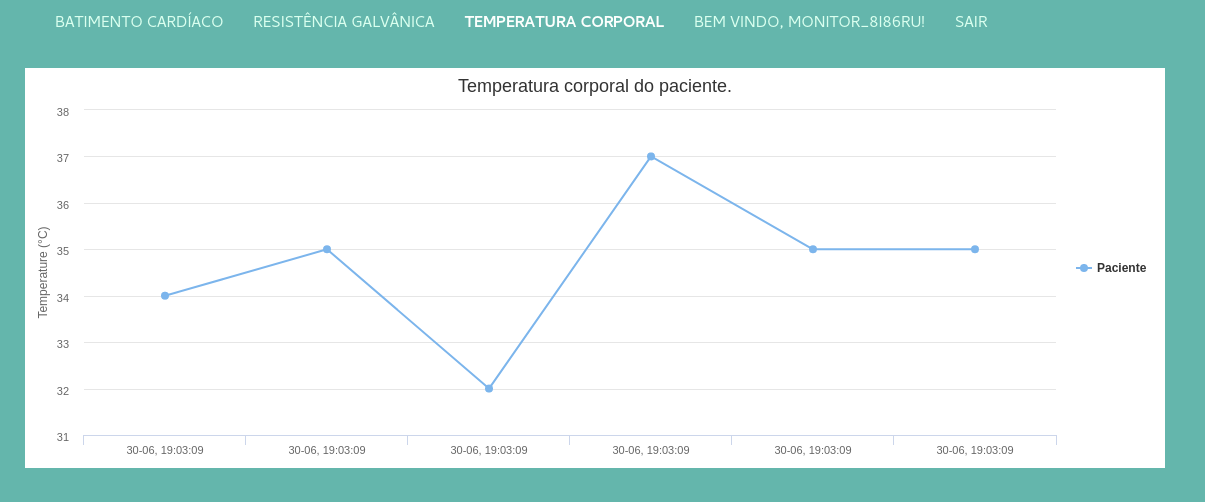
\includegraphics[width=\textwidth]{figuras/wheelshare2.png}
    \end{center}
    \caption{Visualização dos batimentos do paciente no servidor.}
    \label{fig:wheelshare2}
\end{figure}

